%
% File acl2018.tex
%
%% Based on the style files for ACL-2017, with some changes, which were, in turn,
%% Based on the style files for ACL-2015, with some improvements
%%  taken from the NAACL-2016 style
%% Based on the style files for ACL-2014, which were, in turn,
%% based on ACL-2013, ACL-2012, ACL-2011, ACL-2010, ACL-IJCNLP-2009,
%% EACL-2009, IJCNLP-2008...
%% Based on the style files for EACL 2006 by 
%%e.agirre@ehu.es or Sergi.Balari@uab.es
%% and that of ACL 08 by Joakim Nivre and Noah Smith

\documentclass[11pt,a4paper]{article}
\usepackage{apacite}
\usepackage[hyperref]{acl2018}
\usepackage{times}
\usepackage{latexsym}
\usepackage{graphicx}
\usepackage{courier}
\usepackage{hyperref}
\usepackage{courier}
\usepackage [english]{babel}
\usepackage [autostyle, english = american]{csquotes}
\usepackage{gb4e}
\noautomath
\MakeOuterQuote{"}

\usepackage{url}

\aclfinalcopy % Uncomment this line for the final submission
%\def\aclpaperid{***} %  Enter the acl Paper ID here

%\setlength\titlebox{5cm}
% You can expand the titlebox if you need extra space
% to show all the authors. Please do not make the titlebox
% smaller than 5cm (the original size); we will check this
% in the camera-ready version and ask you to change it back.

\newcommand\BibTeX{B{\sc ib}\TeX}

\title{The Role of the QUD in Exhaustivity Inference from Generic Generalizations of Social Groups}

\author{Pratyusha R. Javangula \\
  {\tt pjavan@stanford.edu} \\}

\date{}
\hypersetup{draft}
\begin{document}
\maketitle

\section{Introduction}

As interlocutors communicate over the course of a conversation, their task is complicated by the fact that each of them intends meanings beyond what is said when they make an utterance. Therefore, comprehension is not merely the task of combining fixed lexical word meanings in ways specified by the syntax. Instead, listeners must make judgments about the intended meaning of an utterance that take into account the context in which the utterance was made, as well as more general information about "the way the world is". In order to develop a complete theory of language comprehension, it is imperative to investigate the nature of these judgments, more formally known as pragmatic inferences, and examine the linguistic factors that bring them about. 

Much of the existing literature that seeks to answer questions about how pragmatic inferences arise focuses on a specific type of pragmatic inference known as \textit{scalar implicature}. When making a scalar implicature, a listener infers "some, but not all" from "some" despite the fact that the lexical semantics of "some" taken out of context allows "some" to mean "all" \cite{carston-1998}. However, less research has been conducted into the factors influencing another type of pragmatic inference called exhaustivity inference. Exhaustivity inference is typically defined in the context of question answering and is defined as the inference made by the listener that the speaker's utterance alone constitutes an exhaustive list of answers to the question. For example, if a speaker answers the question "What did you have for dinner?" with "I had a salad," an exhaustive interpretation would be that the speaker \textit{only} had a salad for dinner \cite{vanRooij2004}. 

Exhaustivity inferences are typically drawn from utterances that are answers to questions. However, that question need not be an explicit utterance made over the course of a discourse. Rather, the question being answered could be the more implicit question under discussion. \citet{roberts-1996} defined the question under discussion (QUD) as the question that interlocutors commit to finding an answer for over the course of a conversation. Furthermore, the QUD dictates what alternative meanings are available, given an utterance. For example, for the aforementioned utterance, "I had a salad for dinner," a QUD of, "What did you have for dinner?" proffers different alternative meanings than that of, "What did you do last night?" 

\citet{Frank998} present the Rational Speech Act framework as a means of formalizing the role of the QUD as well as a listener's prior beliefs in pragmatic inference. Under this framework, speakers are assumed to be informative, speakers and listened are assumed to be cooperative with respect to finding an answer for the QUD, and listeners' inferential mechanism is modeled as Bayesian inference. Applied to the generic generalization, "Black lives matter," the framework demonstrated that a pragmatic listener is more likely to draw an exhaustivity inference when they infer the QUD to be "Which lives matter?" rather than "Do Black lives matter?" \cite{degen2017}. Further, \citet{degen2017} determined that a listener's prior beliefs influenced which QUD a listener would infer.

Here we present an empirical investigation into the findings of \citet{degen2017} that the QUD plays a role in exhaustivity inference from utterances that are generic generalizations of social groups. In this case, generic generalizations of social groups are utterances of the form, "\texttt{social group noun} is \texttt{predicate}." To conduct this investigation, we varied the context of generic generalizations via cover stories presented prior to the utterance itself \cite{degen-goodman-2014}. We then asked participants to assess the speaker's beliefs about the extent to which the social group mentioned in the utterance and its complement has the quality explicitly mentioned in the utterance. Finally, participants were asked to report their own beliefs about the extent to which the social groups previously presented have the qualities introduced in the previous utterances. 

We hypothesized that participants would be more likely to draw an exhaustivity inference when presented with an utterance whose cover story induced a QUD of "Which \texttt{social group noun} is \texttt{predicate}?" compared to when presented with an utterance whose contextual cover story induced a QUD of "Is \texttt{social group noun} \texttt{predicate}?" This experiment was pre-registered on the Open Science framework and can be found \href{https://osf.io/hqy94/register/5771ca429ad5a1020de2872e}{here}. 

\section{Method}
\subsection{Participants}
We recruited 160 participants with US IP addresses and at least 95\% of prior HITs approved on Amazon's Mechanical Turk platform (ages: 20-69; mean: 38.9). They were paid 1 dollar.

\subsection{Materials}
\subsubsection{Cover Story Manipulation}
The corpus of stimuli for the cover story manipulation phase comprised 32 combinations of a cover story and an utterance, where each utterance consisted of a social group noun paired with a predicate. 

We selected four pairs of complementary social group nouns: \textit{Democrats and Republicans, men and women, people in their 20's and people in their 50's} and \textit{Europeans and Americans}. We also selected four positively valenced predicates: \textit{competent, rational, polite} and \textit{smart}. Utterances and cover stories containing \textit{Democrats and Republicans} were always combined with the predicate \textit{competent}, those containing \textit{men and women} were always combined with the predicate \textit{rational}, those containing \textit{People in their 20's and People in their 50's} were always combined with the predicate \textit{polite}, and those containing \textit{Europeans and Americans} were always combined with the predicate \textit{smart}. We decided on these specific fixed combinations because they reflect commonly-held stereotypes about each social group. An example utterance presented was the following:

\begin{exe}
\ex\label{string} {Democrats are competent.}
\end{exe}

For each of the four pairs of nouns, we created 8 stimuli. Each of the eight stimuli featured a cover story that evoked one of two QUD's. Each cover story was about a speaker in a meeting at their place of work with the larger group of people they work with, where a secondary actor announces that they will be choosing one or two subgroups for a project based on the extent to which the group(s) is/are \texttt{predicate}. Depending on if the secondary actor would be choosing one or two subgroups, the story induced an implicit QUD that made it relevant either that the speaker's utterance that "\texttt{social group noun} is \texttt{predicate}" should be pragmatically strengthened to "Only \texttt{explicitly mentioned group noun} is \texttt{predicate}" (\textit{who?} condition) vs. "\texttt{explicitly mentioned noun} is \texttt{predicate}, and the extent to which \texttt{complementary noun} is \texttt{predicate} is not at issue" (\textit{are?} condition). A cover story inducing the \textit{who?} QUD follows:

\begin{exe}
\ex\label{string} {Michelle is a senator of a major political party and is a member of many legislative committees. Every legislative committee is composed of either all Democrats or all Republicans. The other day in a Senate session, the head of the Senate unveiled that he would be choosing an existing legislative committee to work on a new project based on their competence.}
\end{exe}

Now, we present an example cover story inducing the \textit{are?} QUD: 

\begin{exe}
\ex\label{string} {Michelle is a senator of a major political party and is a member of many legislative committees. Every legislative committee is composed of either all Democrats or all Republicans. The other day in a Senate session, the head of the Senate unveiled that he would be choosing two existing legislative committees to work on a new, highly classified project based on their competence, and that he had already chosen one team of Democrats.}
\end{exe}

The cover story in each stimulus had either a male or female speaker and an opposite-gender secondary actor (e.g. \textit{head of the Senate}). Finally, in each of the eight stimuli, the critical utterance explicitly mentions one of the two social group nouns in the pair. 

\subsubsection{Prior Beliefs Collection}

The corpus of stimuli for the prior beliefs collection phase comprised eight questions of the format "How \texttt{predicate} do you find \texttt{social group noun}?" An example follows: 

\begin{exe}
\ex\label{string} {How smart do you find Americans?}
\end{exe}

Stimuli were created by combining each of the eight nouns presented in the cover story manipulation phase with the predicate to which they were fixed.

\subsection{Procedure}
\subsubsection{Cover Story Manipulation}
Each participant was presented with a random one from each of the four sets of eight stimuli. Therefore, in total each participant responded to four stimuli, one for each pair of social group nouns. An important caveat to the random selection was that we presented two stimuli with cover stories inducing the \textit{who?} QUD and two with cover stories inducing the \textit{are?} QUD, such that QUD was a within-participants manipulation. Trial order was randomized between-participants. 

First, participants were presented with the cover story and asked to read it in its entirety. Then, to ensure that participants paid attention to the story, they had to answer the following comprehension question: \textit{Has the} \texttt{secondary actor} \textit{chosen at least one} \texttt{subgroup}? They were only allowed to proceed once they correctly answered the question. The correct answers were either \textit{yes} if the cover story induced the \textit{are?} QUD or \textit{no} if the cover story induced the \textit{who?} QUD. 

They were then asked \textit{How }\texttt{predicate } \textit{are }\texttt{social group noun}\textit{, according to }\texttt{speaker}\textit{?} They then adjusted two sliding scales with endpoints labeled “extremely \texttt{opposite of predicate}” and “extremely \texttt{predicate}” to indicate their judgments of the speaker's beliefs of both the group noun in the utterance and its complement. Slider values were recorded as falling between 0 (''extremely \texttt{opposite of predicate}'') and 1 (''extremely \texttt{predicate}'').

\begin{figure}[h]
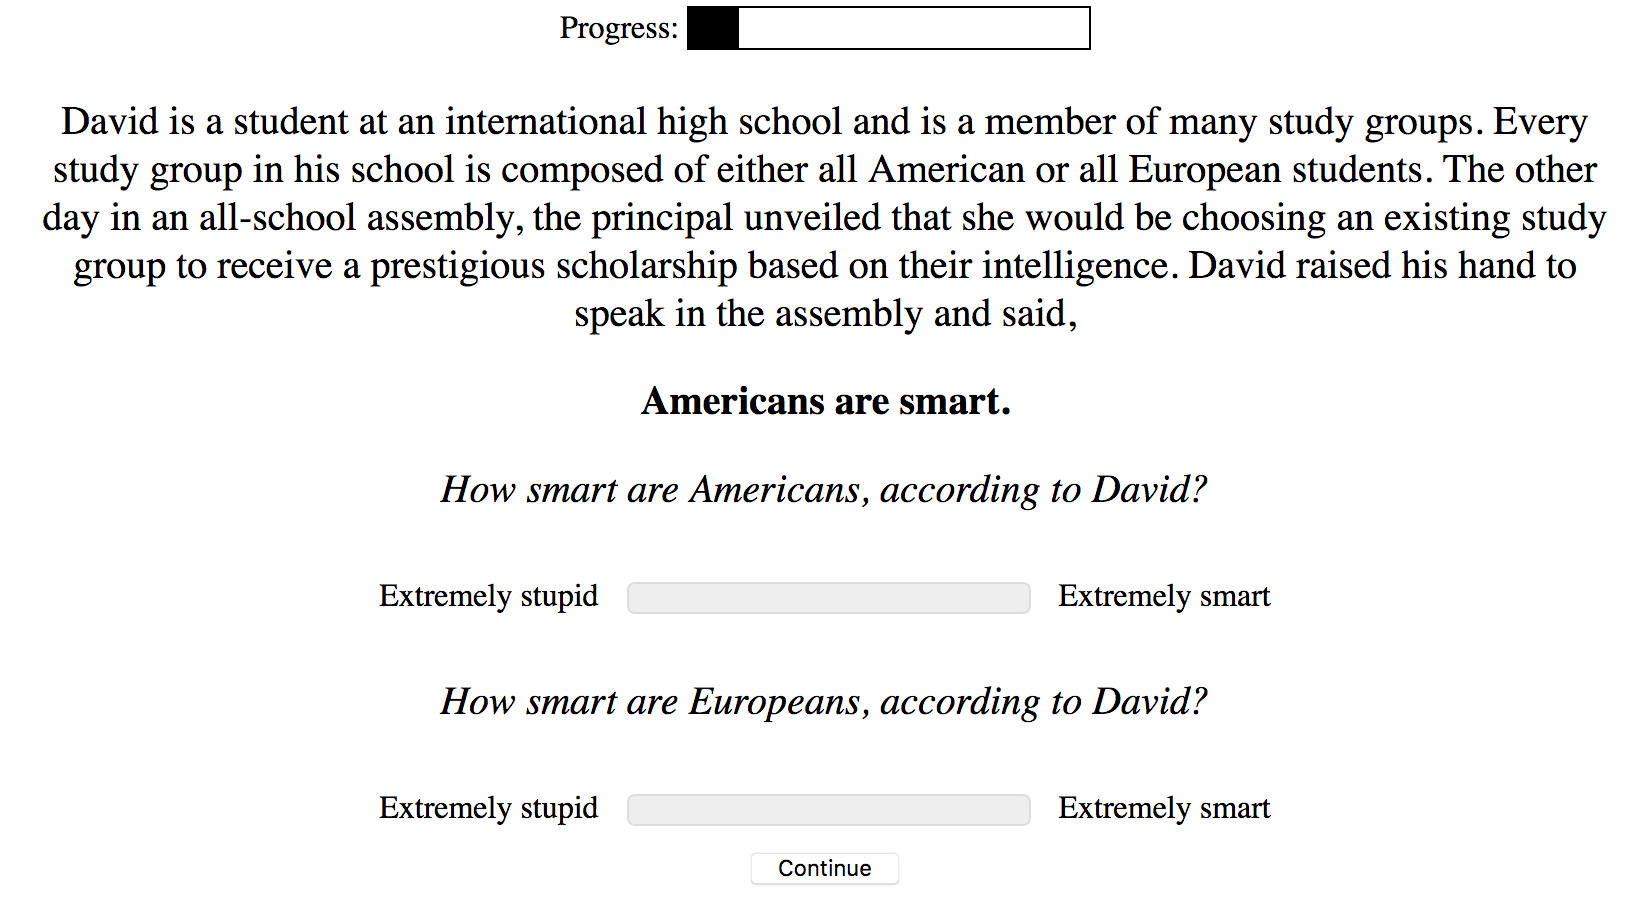
\includegraphics[width=\linewidth]{trial.png}
\caption{Distribution of gender over samples in training data set.}
\label{trial}
\end{figure}

For our purposes, the opposite of \textit{smart} is \textit{stupid}, the opposite of \textit{rational} is \textit{emotional}, the opposite of \textit{polite} is \textit{rude}, and the opposite of \textit{competent} is \textit{incompetent}. Figure \ref{trial} presents a screenshot of a standard cover story manipulation trial.

If an exhaustivity inference is drawn, meaning that the speaker is interpreted as saying that only the critical noun from the utterance is \texttt{predicate}, participants should judge that group noun as having a greater value for \texttt{predicate} than the complementary group noun. If instead they do not draw an exhaustivity inference, the difference in their judgments for the extent to which each group is \texttt{predicate} should be smaller.

\subsubsection{Prior Beliefs Collection}
Each participant was presented with each of the eight stimuli created for the prior beliefs collection phase. Trial order was randomized between-participants. 

They asked \textit{How }\texttt{predicate } \textit{do you find }\texttt{social group noun}\textit{?} They adjusted two sliding scales with endpoints labeled “extremely \texttt{opposite of predicate}” and “extremely \texttt{predicate}” to indicate their responses for both the group noun in the utterance and its complement. Slider values were coded in the same way as for the cover story manipulation phase.

\begin{figure}[h]
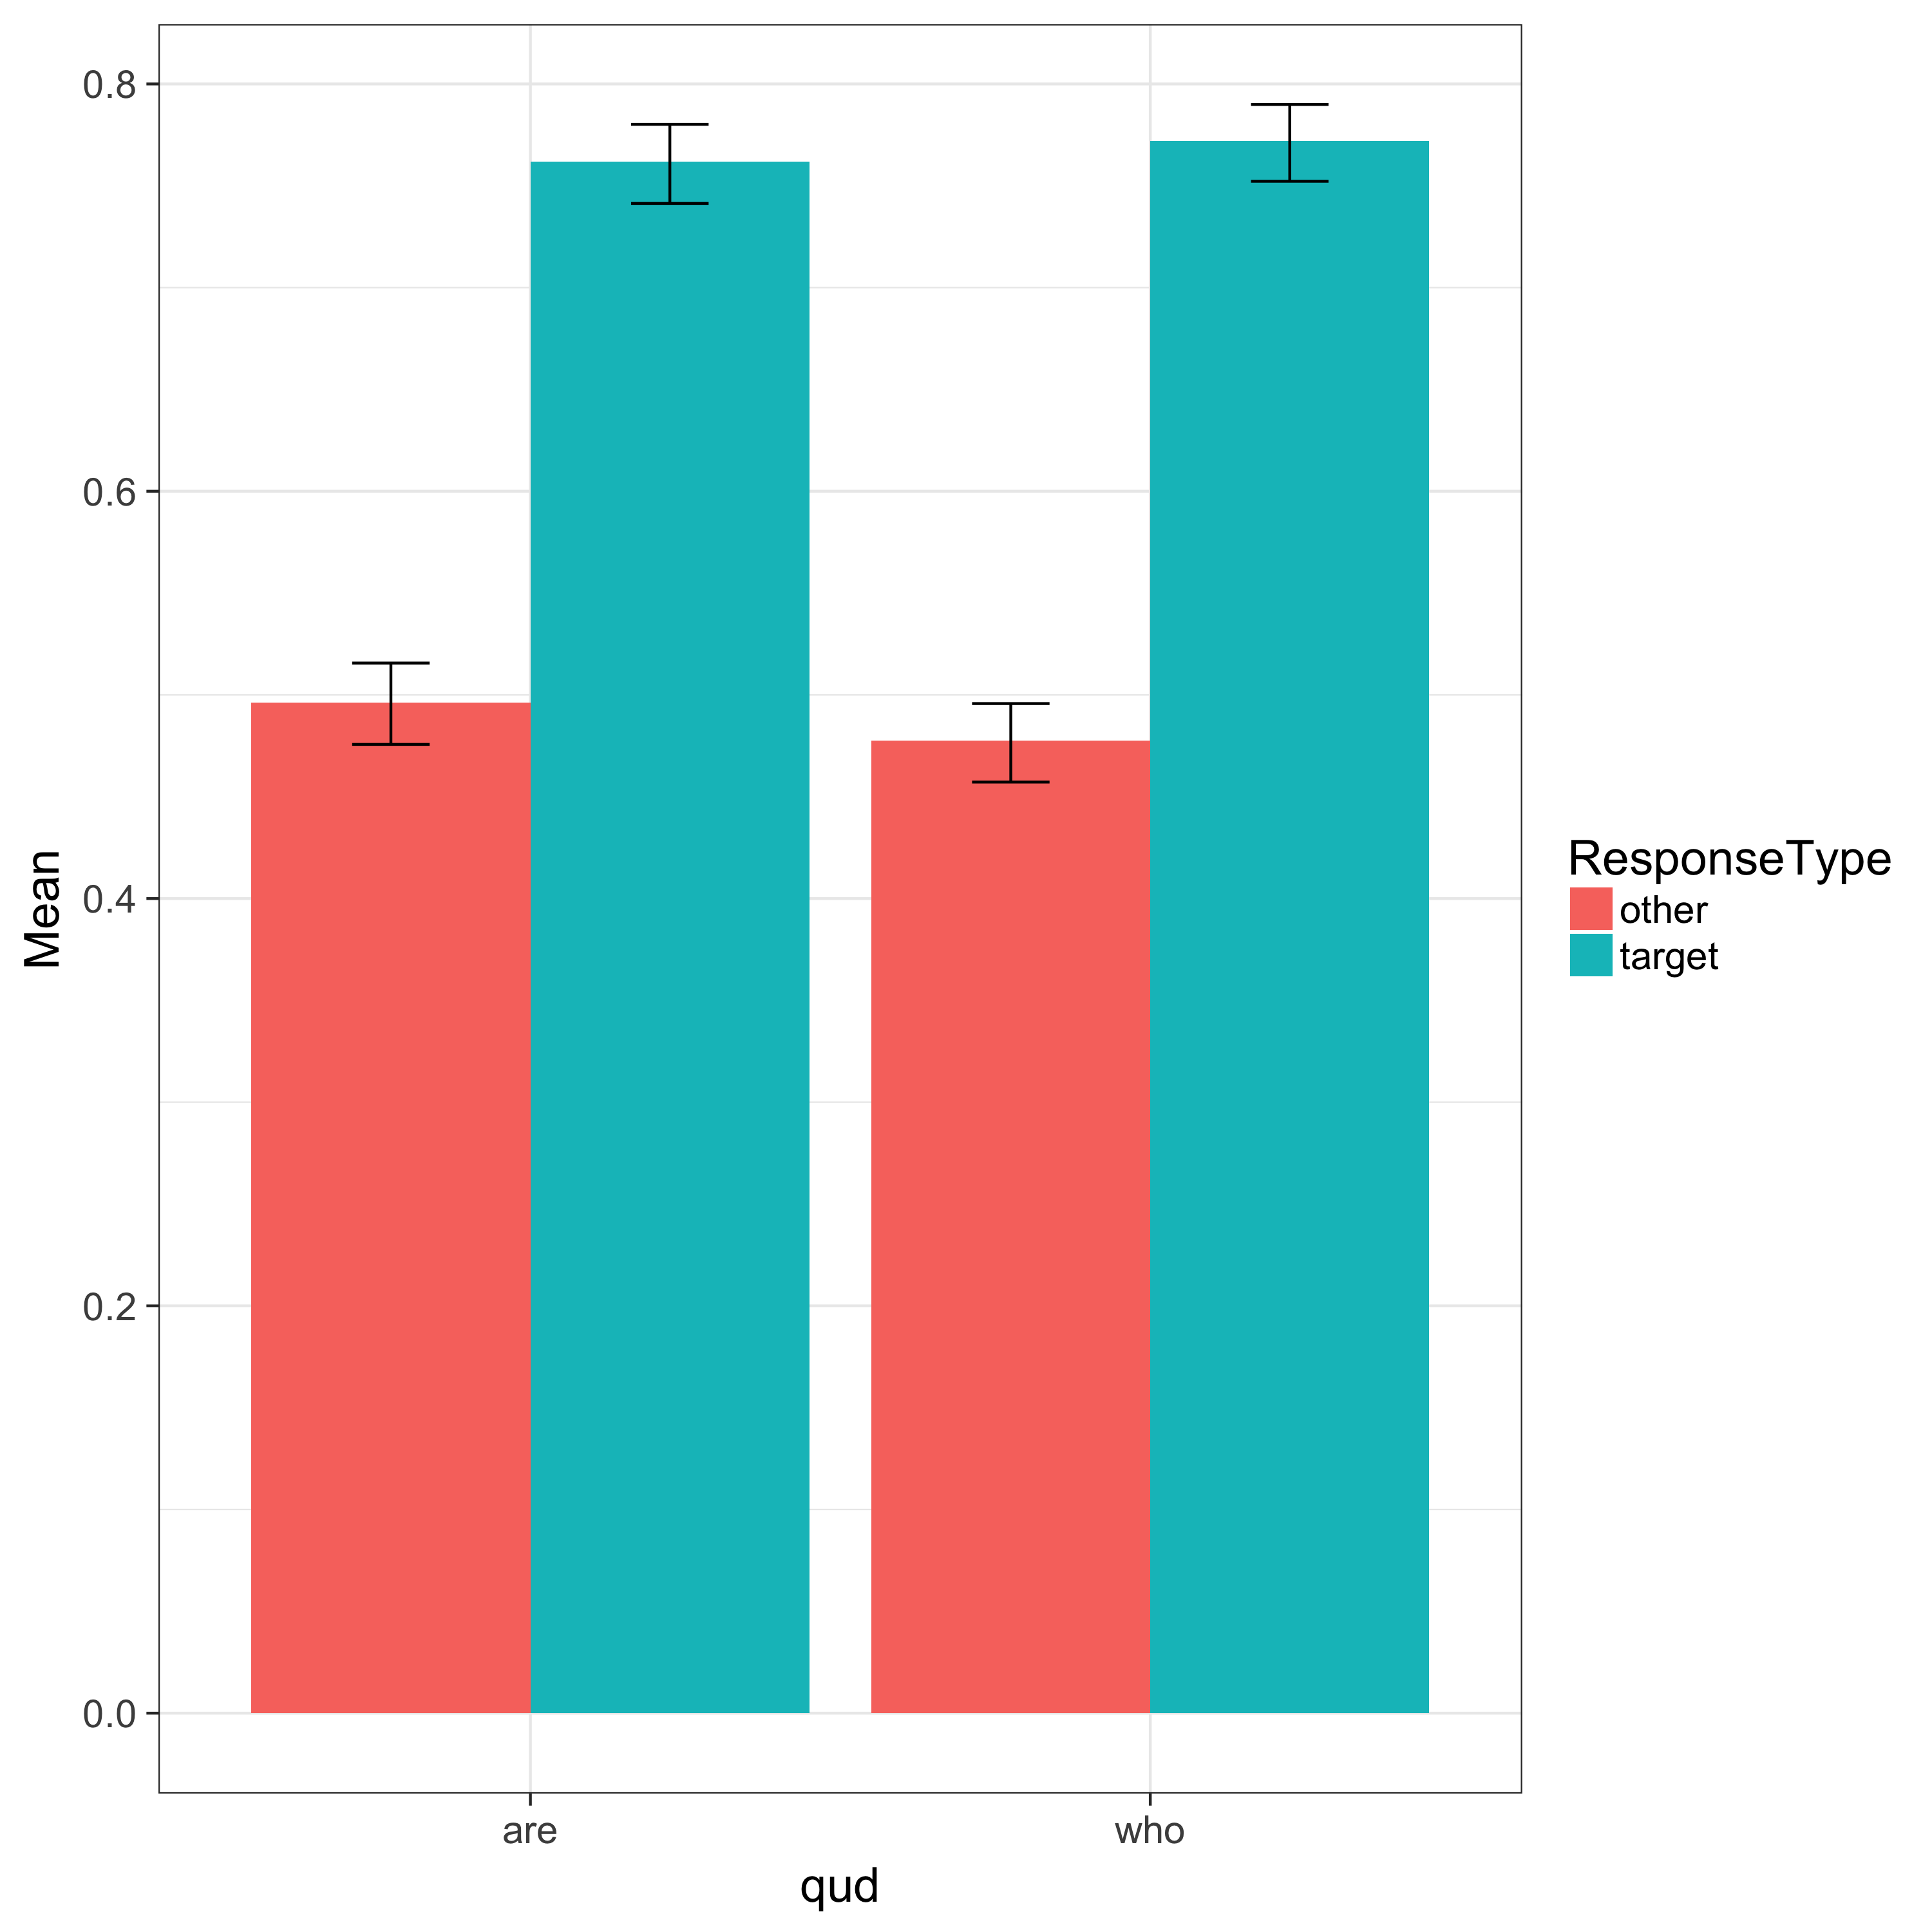
\includegraphics[width=\linewidth]{qud_means.png}
\caption{Mean response to as a function of QUD to target and other social group noun.}
\label{means}
\end{figure}
\section{Results}

Mean slider response of target social group noun (mentioned directly in the utterance) and the other social group noun (its complement) as a function of the context-induced QUD are shown in Figure \ref{means}. A visual assessment of the difference in mean response between \textit{who?} and \textit{are?} conditions seems to suggest that in line with our predictions, there is a marginally smaller difference between mean response for the target and other nouns in the \textit{are?} condition compared to the \textit{who?} condition. However, this difference does not suggest a significant effect of QUD manipulation. There does appear to be a significant difference between mean response for the target social group noun and the other social group noun.

\begin{figure}[h]
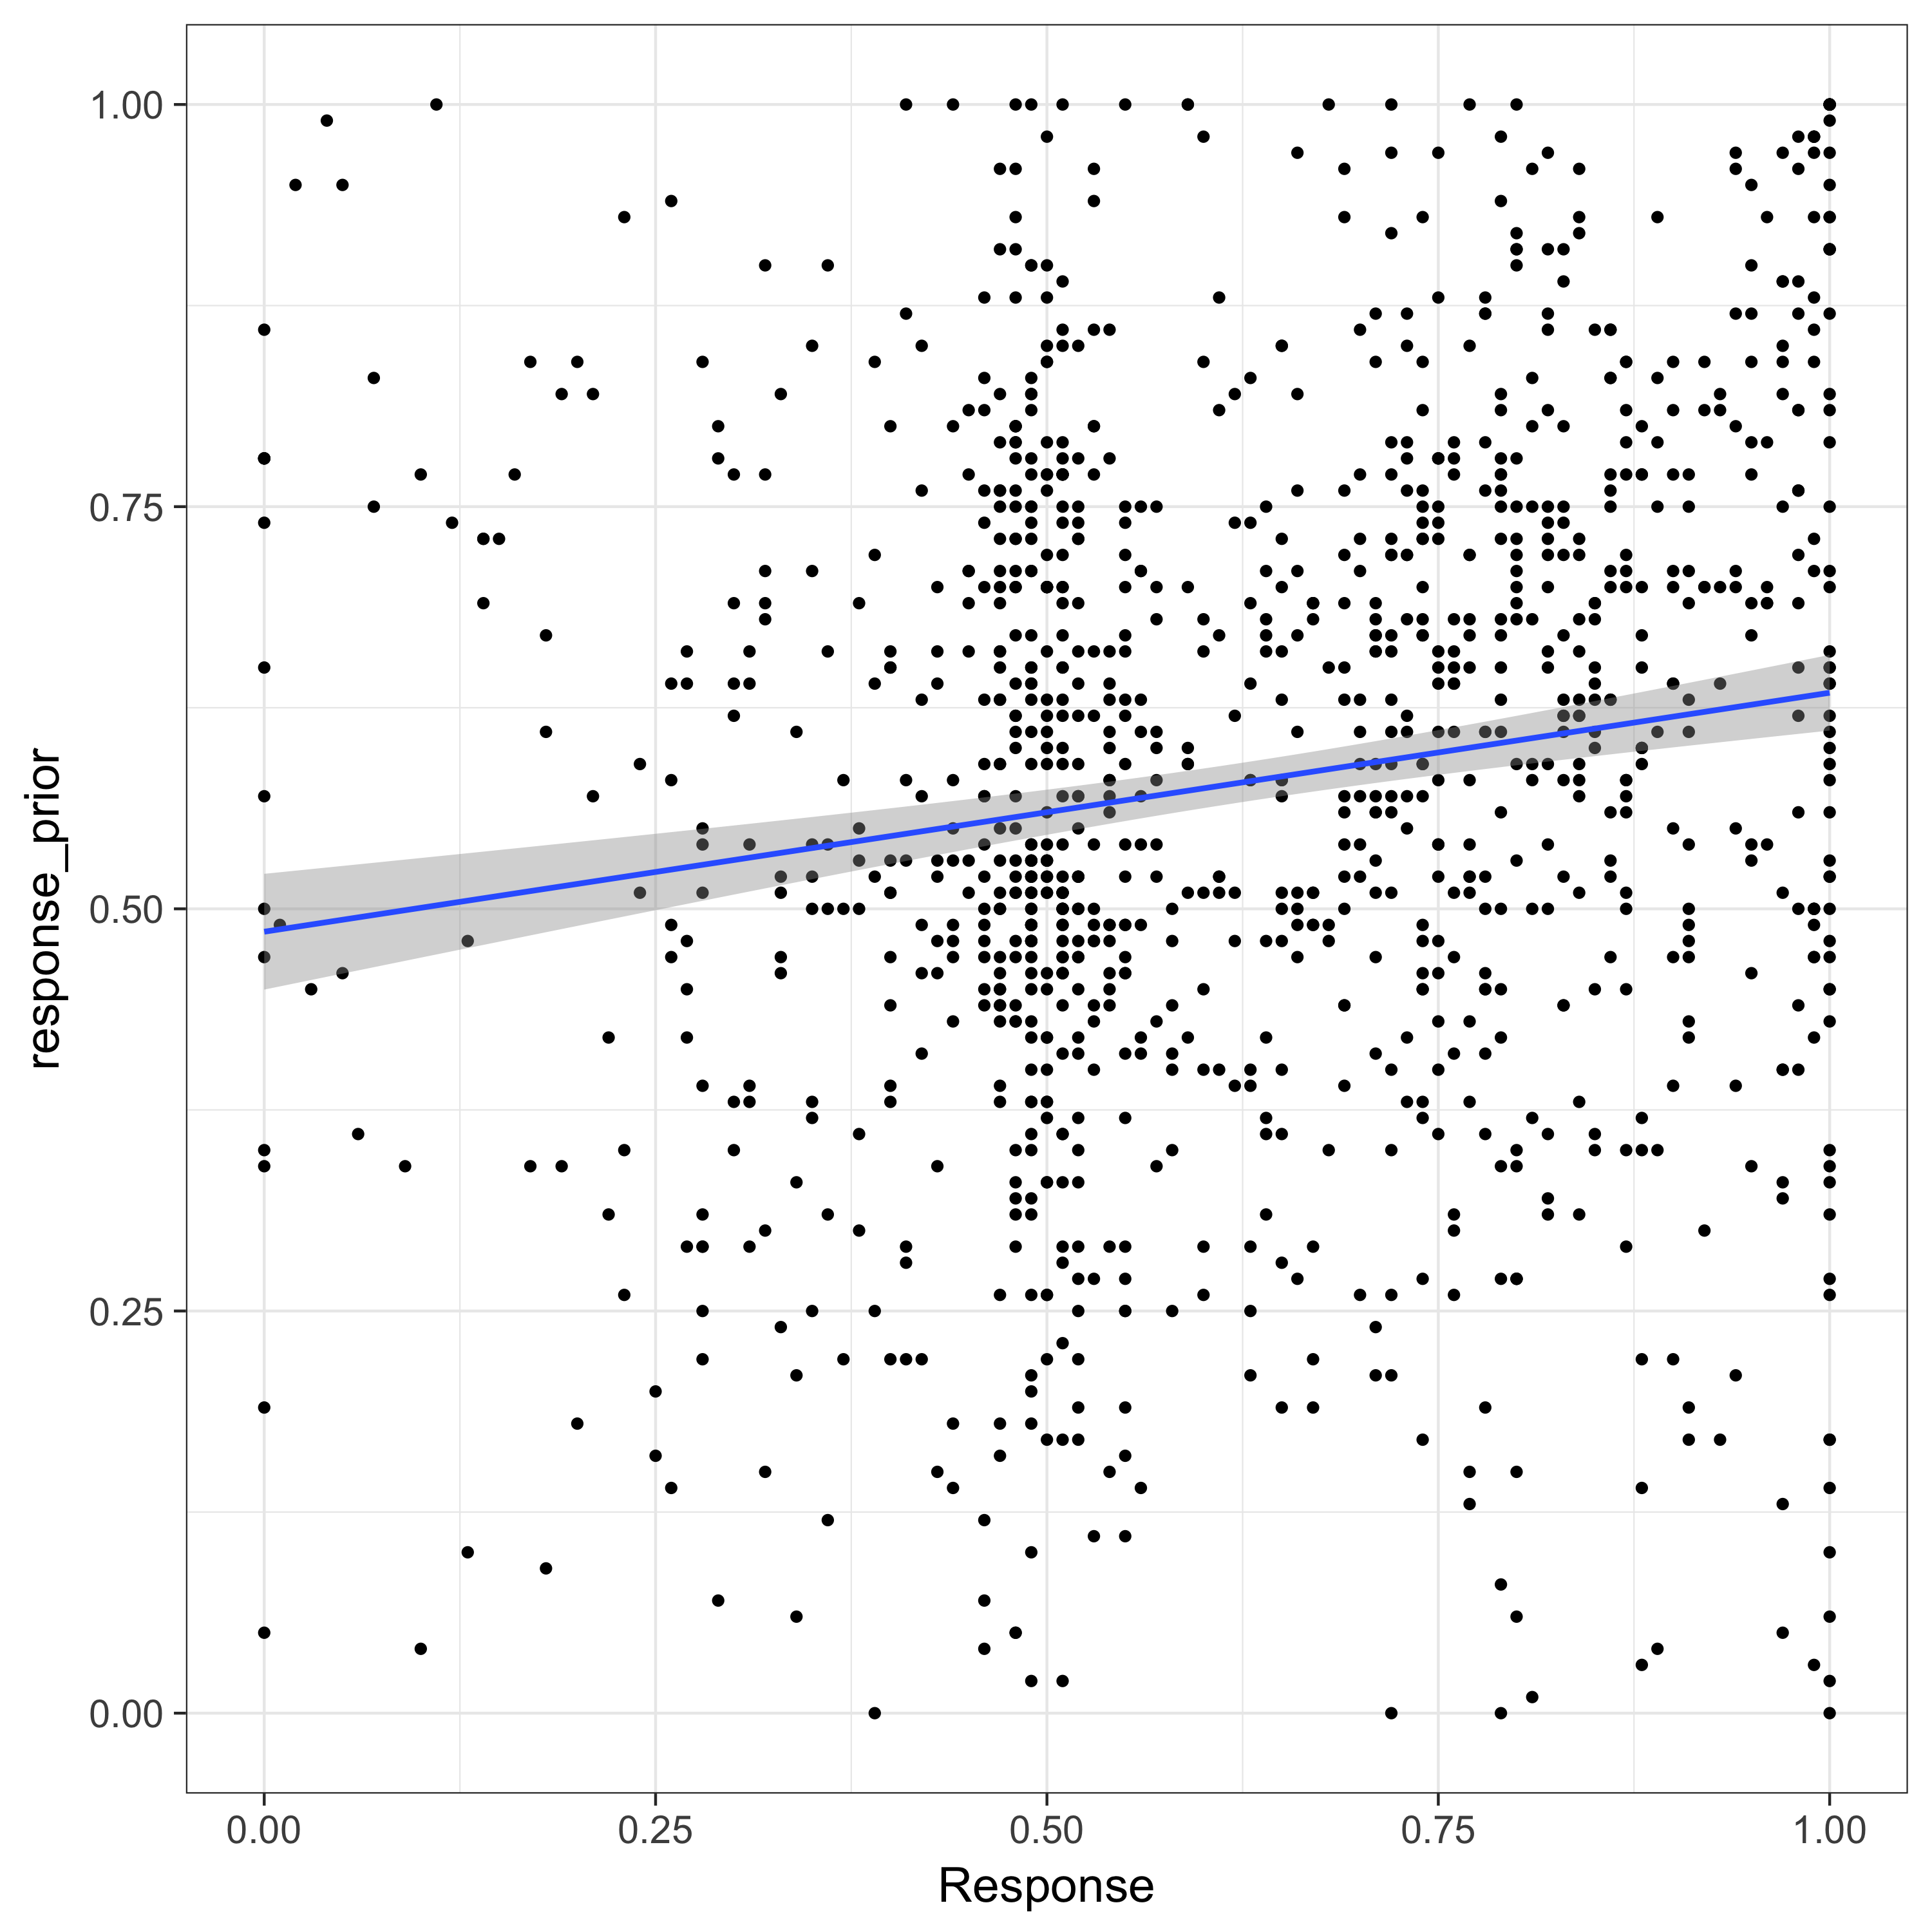
\includegraphics[width=\linewidth]{priors_responses.png}
\caption{Response to noun (target and other) as a function of prior belief.}
\label{priors}
\end{figure}

We also investigated whether participants' assessments of the speaker's beliefs of the target social group noun and other social group noun were related in any way to their own beliefs. Figure 3 presents participant prior beliefs as a function of their judgments of the speaker's beliefs, with a linear smoother and 95\% confidence intervals. 

Examining the slope of the linear smoother shows a slightly positive correlation between a participant's judgment of the speaker's beliefs about a social group noun and a participant's own belief about that social group noun. To verify the conclusions made from inspection of Figure \ref{priors}, we conducted a Pearson correlation between judgments of the speaker's beliefs and found that they were weakly but significantly correlated, $r$(1200) $= 0.1557$, $p < .001$.

After observing this significant correlation, in addition to investigating the effect of QUD manipulation on participant judgments of speaker beliefs, we sought to address the additional question of the role that prior beliefs play in judgments of speaker beliefs, if any.  

To address these questions, we conducted a Bayesian generalized multivariate non-linear regression using the \texttt{brms} package \cite{buerkner}. Our purpose for using Bayesian methods was that it would allow us to fit a model with a full random effects structure where mixed-effects linear models instantiated using \texttt{lme4} would not. 

The model predicted the log odds of slider response representing a participant's judgment of the speaker's beliefs about the extent to which \texttt{social group noun} is \texttt{predicate} from fixed effects of the QUD, response type (whether the response given is in reference to the critical noun versus the other noun), their interaction, and the participant's prior beliefs. In order to avoid problems related to collinearity, we centered all predictor variables. We included the maximal random effects structure justified by the design: random by-participant and by-item slopes for the interaction between QUD and response type and the prior belief (reflecting the possibility that the effects of these variables could vary by participant and by item). Four chains converged after 2000 iterations each (warmup = 1000, \(\hat{R}=1\) for all estimated parameters). T 

We report 95\% confidence intervals and the posterior probabilities $P(\beta > 0)$ that coefficients for QUD, response type, their interaction, and prior beliefs are greater than zero. We also provide 95\% confidence intervals (CI) of the posterior distributions for each coefficient.  Finally, if zero is not included in the CI for the posterior distribution of a variable's coefficient, we have strong reason to believe it has a significant effect on slider response. So too, if $P(\beta > 0)$ is close to zero or one.

\begin{table*}
\centering
\begin{tabular}{llll}
  Variable & $\beta$ & 95\% CI&$P(\beta) > 0$\\
  \hline
  QUD & $0.00$ & {[}-0.03,0.02{]} &$0.2331$\\
  response type & $-0.28$ & {[}-0.33,-0.24{]} &$0$\\
  QUD * response type & $-0.03$ & {[}-0.08,0.02{]} &$0.1015$\\
  prior beliefs & $0.09$ & {[}0.03,0.16{]} &$0.9963$\\
\end{tabular}
\caption{Posterior mean $\beta$, 95\% confidence interval, and $P(\beta) > 0$ for all fixed effects and interactions.
  }
\end{table*}

\begin{figure}[h]
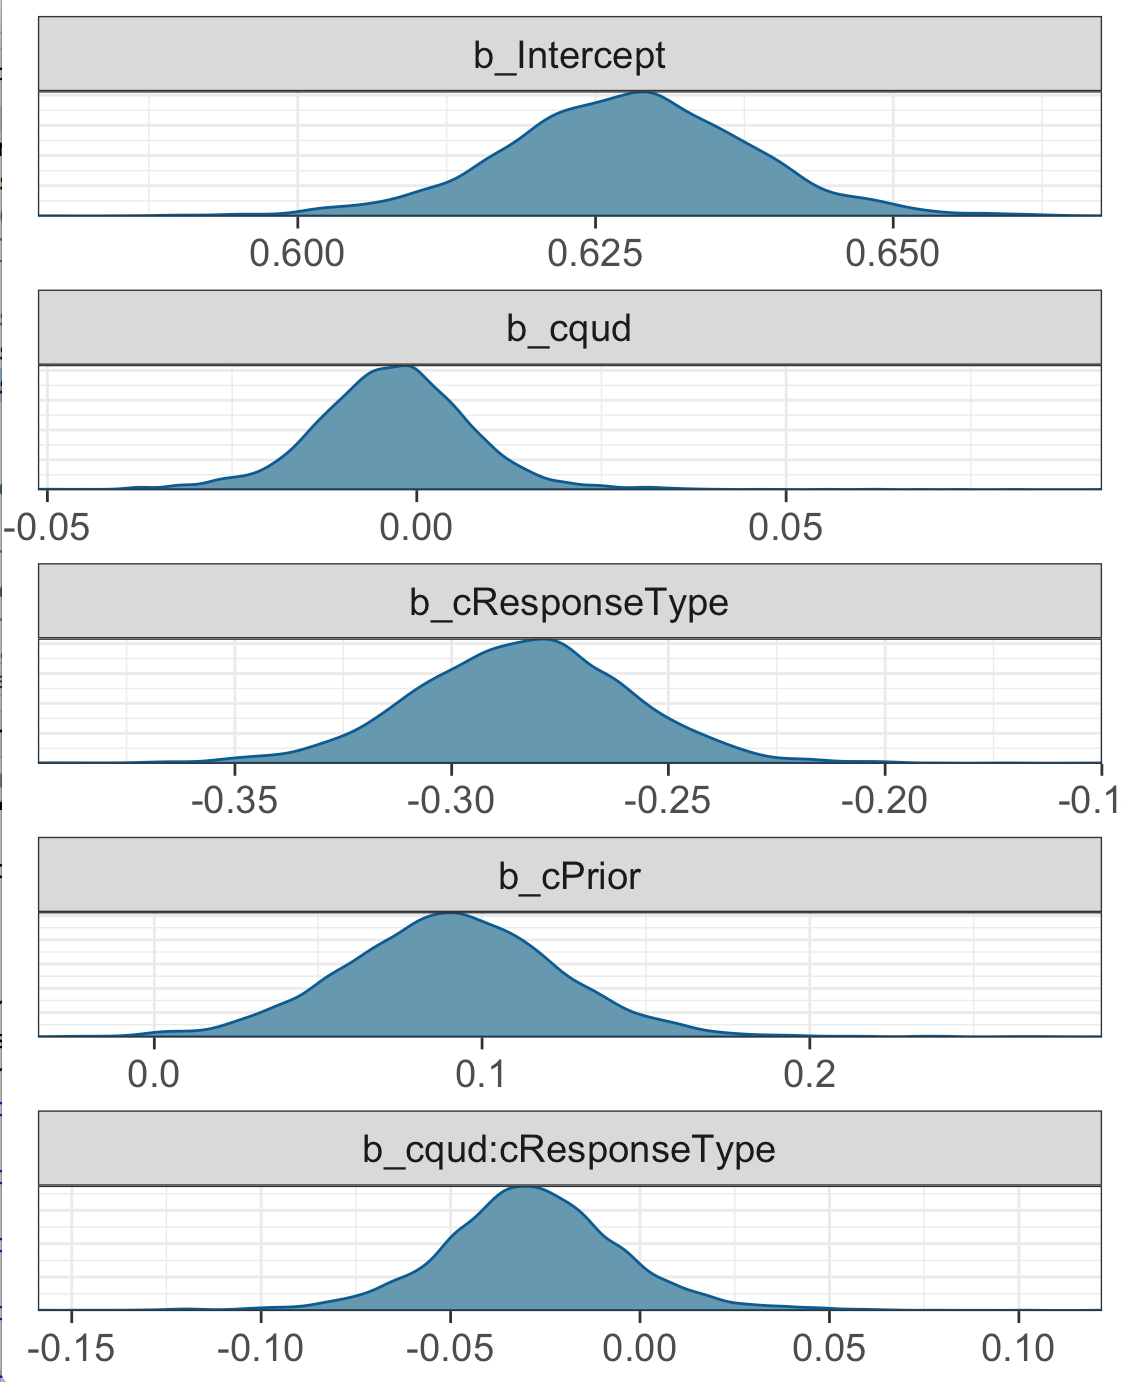
\includegraphics[width=\linewidth]{beta.png}
\caption{Posterior distributions for all \betas of model predictors.}
\label{nounclass}
\end{figure}


Table 1 presents posterior mean $\beta$, 95\% CI, and $P(\beta > 0)$ for each of the predictors to the model, and Figure 4 presents the posterior distributions of the coefficients of each predictor. From Table 1 and Figure 4 together it is clear that there is a significant effect of response type and prior, but no significant effect of QUD and no significant interaction. These results align with the intuitions obtained from examining the data visualizations. Nevertheless, we find that our original predictions that QUD would have a significant effect on participant judgments of speaker beliefs were not borne out. We interpret these results, reason about their origins, and propose future directions in the next section. 

\section{Discussion}

The purpose of the present research was to assess whether there is empirical evidence to support the finding from previous work using computational tools to model pragmatic inference that inferred QUD has an effect on exhaustivity inference in response to generic generalizations of social groups. This aim was carried out by presenting participants with a series of utterances that were generic generalizations of different social groups, accompanied by cover stories intended to spur the participant to infer one of two QUDs. We then recorded participants' judgments of the speaker's beliefs about the extent to which the social group implicated in the utterance and its unmentioned complement embody the predicate of the utterance. Finally, we collected participants' prior beliefs about the extent to which each of the previously presented social groups embodies the predicate it was fixed to in the previous phase. 

Prior to conducting this research, we operationalized an exhaustivity inference as a large difference between a participant judgment of a speaker's beliefs about the social group explicitly mentioned in the utterance and its unmentioned complementary social group. We hypothesized that when presented with a cover story inducing the \textit{who?} QUD, participants would be more likely to draw an exhaustivity inference than when they were presented with a cover story inducing the \textit{are?} QUD. 

The empirical pattern of obtained results is as follows. We observed effects of response type and priors on participant judgment of speaker beliefs of the extent to which a certain social group embodies a given predicate. On the other hand, we did not observe an effect of QUD or of the interaction between QUD and response type. 

Although not hypothesized, the observed main effect of response type validates the study design. Since participants gave significantly different responses for the target social group noun compared to the unmentioned other social group noun, we can conclude that our cover story and utterance presentation appropriately informed participants that the the extent to which the two groups embodied the predicate are different. 

Examining the pattern of results in Figure \ref{means}, however, it is surprising that in the \textit{are?} condition, there is such a large difference between the responses to target and other nouns. Since the \textit{are?} QUD is intended to prime participants to believe the complementary social noun is irrelevant, and there is no utterance explicitly mentioning the complementary social noun, it is surprising that participants gave low judgments to the other noun, on average. We suspect this phenomenon arose because all participants were not uniformly inferring the correct QUD across all trials. In future work, we aim to employ the approach taken by \citet{degen-goodman-2014} and explicitly include a comprehension question to ensure correct interpretation of the QUD from the cover story. 

Similarly, the observed main effect of prior beliefs on slider response was not hypothesized. We find it reasonable that a participant's own prior beliefs would have an effect on their judgments of a speaker's beliefs. Furthermore, these results reaffirm the findings of \citet{degen2017} that prior beliefs have a role to play in pragmatic inference from generic generalizations of social groups. 

Most importantly, there was no observed effect of QUD, which contradicts the hypotheses formulated prior to conducting the experiment. In discussing why we believe these results may have arisen, we will address a major limitation of this work.

Aside from the aforementioned limitation that participants may not have inferred the correct QUD for the condition they were assigned to in a particular trial, we believe these results came about due to the nature of the interaction between the social group noun and predicate in certain utterances. 

\begin{figure}[h]
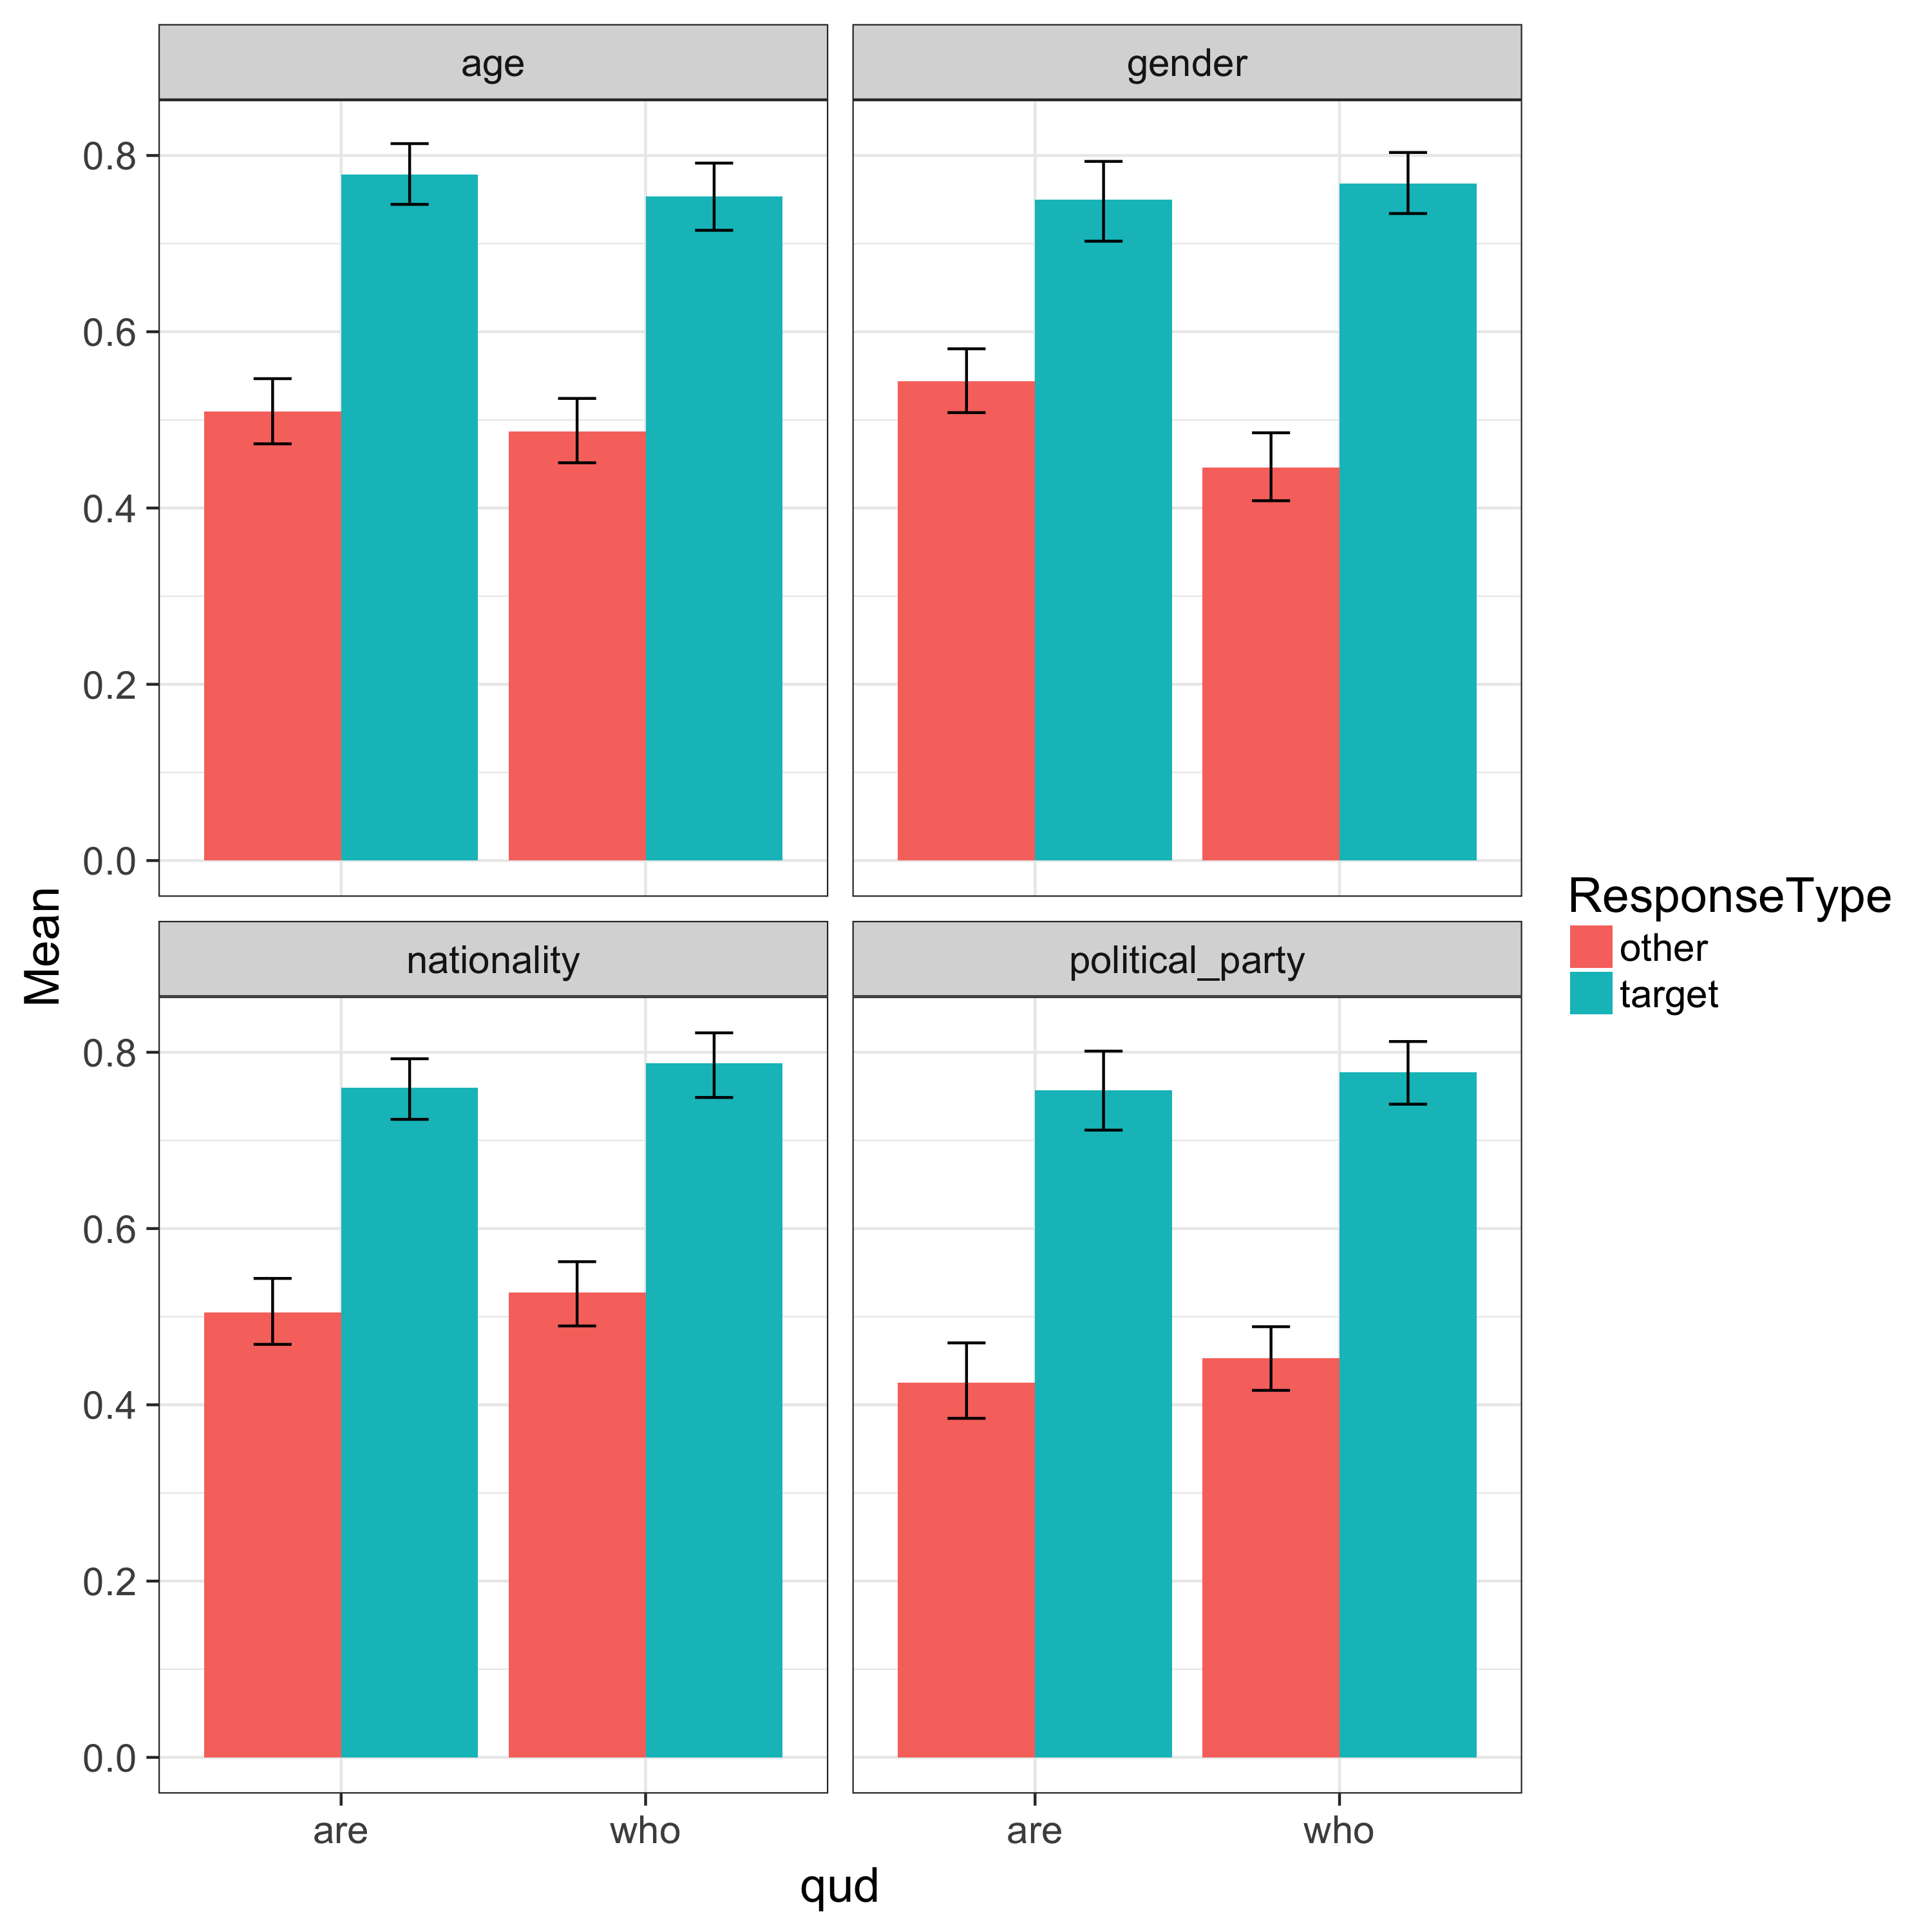
\includegraphics[width=\linewidth]{qud_means_nounclass.png}
\caption{Mean response to as a function of QUD to target and other social group noun.}
\label{nounclass}
\end{figure}

Figure \ref{nounclass} presents mean response as a function of QUD to the target and complementary noun, separated by pair. From Figure \ref{nounclass} we can see that the hypothesized effect of QUD occurs when participants responded to utterances about men or women, but not for utterances about any other social group nouns. 

This item-specific effect may have arisen because each of the generic generalizations of social groups may have been assigned a different meaning, regardless of the cover story that accompanied it. \cite{tessler-goodman} found that generic statements like "Dogs bark" and "Robins are female" take into account diverse sets of prior beliefs about different properties for each statement and thus are interpreted vastly differently in and out of context. 

The question of how meaning is assigned to statements of this nature about social groups is relatively unexplored. Thus, in order to meaningfully explore the role of the QUD in exhaustivity inference of these types of utterance, it will be necessary to extend the findings of \cite{tessler-goodman} to utterances like those that we presented as stimuli in the current work.

In light of the vastly different results for different items, future work must prioritize an investigation of how existing pragmatic theories of generic language apply to generic statements about social group nouns, as well as a separate investigation of the role of the QUD in exhaustivity inference of non-generic statements like "I had a salad for dinner."

\section{Conclusion}
We have shown that overall, presentation of different cover stories meant to evoke different QUD's prior to an utterance plays no role in exhaustivity inference of generic generalizations of social groups. However, we were able to show that a participant's prior beliefs, as well as the fact of whether a participant gave a response about an explicitly mentioned or complementary social group noun, can greatly affect a participant's judgment of speaker beliefs about both the noun in the utterance and the complementary noun. 

\section*{Acknowledgments}

Many thanks to Judith Degen for advising this work and to students of Linguistics 245 for their invaluable feedback and support.

% include your own bib file like this:
%\bibliographystyle{acl}
%\bibliography{acl2018}
\bibliographystyle{apacite}
\bibliography{acl2018.bib}

\end{document}
